\chapter{OpenStack Folsom}\label{cap:openstack}

\noindent The current section intends to detail the IaaS Cloud implementation that has been chosen: OpenStack. Initially, a global vision will be given to the reader, to progressively focus on its constituents modules' responsibilities and how they collaborate to maintain the service running.

\section{Global Architecture}\label{sec:arquitecturaglobal}

\noindent Figure \ref{fig:arquitecturaos} shows the three basic operational components of OpenStack Folsom:

\begin{description}
 \item[Functional Core:] OpenStack Compute, OpenStack Quantum and OpenStack Storage (Cinder and Swift).
 \item[Web Management Interface:] OpenStack Horizon.
 \item[Shared Services:] OpenStack Glance, OpenStack Keystone and other related services like a DBMS for persisting meta-data or a messaging queue.
\end{description}

\begin{figure}[tbp]
\begin{center}
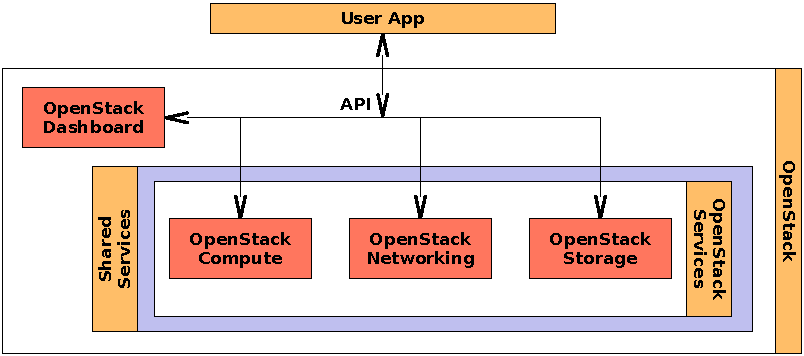
\includegraphics[width=0.9\textwidth]{imagenes/012.pdf}
 \caption{OpenStack Arquitecture}
\label{fig:arquitecturaos}
\end{center}
\end{figure}

The different components have been devised in a shared nothing fashion. This provides the cloud admin the flexibility required to distribute the modules over the cluster as pleased. An example of a particular OpenStack deployment is shown in figure \ref{fig:despliegueos}; OpenStack's own modules are displayed in red, supporting services are shown in violet. What it is missing from the diagram, for clarity, is the asynchronous queue that mediates inter-module communication. Qpid and RabbitMQ are the two queue implementations that are officially documented, being the former the one that we used in our test deployment.

\begin{figure}[tbp]
\begin{center}
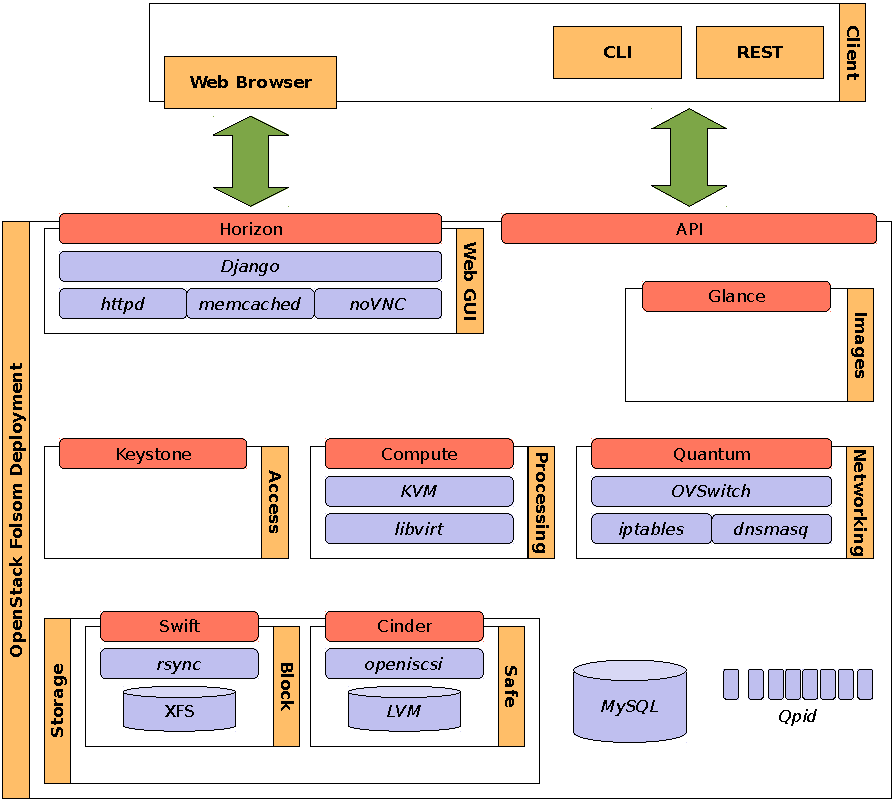
\includegraphics[width=0.99\textwidth]{imagenes/011.pdf}
 \caption{Example of an OpenStack Folsom deployment}
\label{fig:despliegueos}
\end{center}
\end{figure}

\section{Horizon}\label{sec:horizon}

\noident Horizon represents the fundamental window to set up the cloud. As discussed in the previous section, Horizon does not currently --- as of Folsom version --- present a global view of the physical infrastructure, leaving the user in the dark in this respect. Horizon is written in Python on top of \texttt{Django}, the web framework. Django itself relays on a web server like \texttt{httpd} to expose static files, uses a caching mechanism (\texttt{memcached}) to speedup load times and a terminal embedding (\texttt{noVNC}) system to view the output of the virtual graphic card directly on Horizon.

To manage and create instances in the cloud, OpenStack gives the cloud admin the ability to register authorization roles that will let the users consume those services whose role give access to. While the admin is allowed to sign up custom roles, two roles that ship the distribution are the \emph{Cloud Admin} and the \emph{Cloud Member}.

A user granted the admin role will be able to manage:

\begin{description}
 \item[Tenants:] Create, delete, member users, alter quotas, etc.
 \item[Users:] Create, modify or delete.
 \item[OS Images:] List, remove or modify meta-data.
 \item[Instances:] Reset, shutdown, suspend, print log on screen, etc.
 \item[Volumes:] Create, list, attach to an instance, etc.
 \item[Networks:] Create, modify or delete.
\end{description}

A user granted the member role will be able to:

\begin{description}
 \item[Status:] Quota, resources, etc.
 \item[Instances:] create, shutdown, reset, suspend, print log, create image from a running instance (snapshot), etc.
 \item[Volumes:] List, create, modify, attach to an instance, create a volume snapshot, etc.
 \item[Images:] Create, list, delete, modify, etc.
 \item[Networking:] Manage public IPs (floating IPs).
 \item[Security groups:] Create, delete or modify security rules.
 \item[Keypairs:] Create, modify or delete.
\end{description}

\section{Keystone}\label{sec:keystone}

\noindent Keystone is the central security check point and information repository storing information needed to access the cloud installed services. It verifies, before each request, user credentials and authorizations in OpenStack services. Keystone divides this functionality in two parts: on the one hand user control, on the other service catalog.

To deal with users, Keystone assigns them tenants or projects. Users, as discussed above, are granted the membership to a tenant and a service quota they will have to adhere to; they are also restricted to the tenant quota.

To organize the catalog at hand Keystone defines two other concepts within the service catalog: \emph{Services} and \emph{endpoints}. A service in the catalog is a mere abstract description of an exploitable cloud feature by the user. The particular implementation of the service is managed by the set of endpoints associated to it. Said collection contains every piece of information that is required for users to consume the services. Figure \ref{fig:secuenciais} shows a Sequence Diagram portraying the interchanged messages between the different entities taking part to consume a service: \emph{Create a new instance}.

\begin{figure}[tbp]
\begin{center}
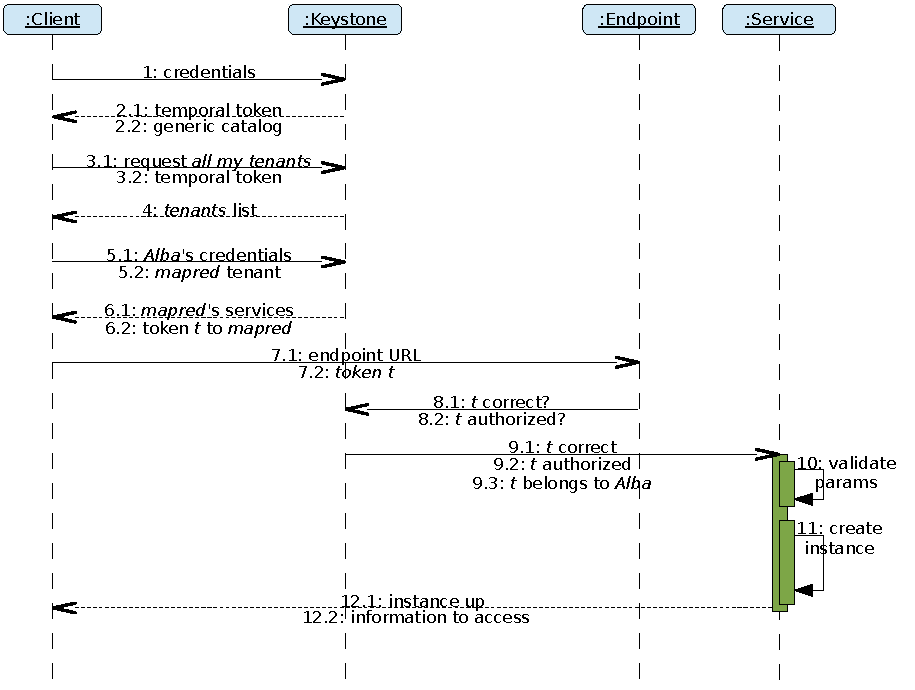
\includegraphics[width=0.99\textwidth]{imagenes/013.pdf}
 \caption{Sequence Diagram --- create instance}
\label{fig:secuenciais}
\end{center}
\end{figure}

Stemming from the fact the Horizon exposes only a part of OpenStack functionality, to help dealing with security Keystone installs a CLI tool to interact with the REST service in charge of administrative operations. Issuing certain commands to Keystone through a terminal requires the knowledge of the admin token, which has to be conveniently secured, or the login credentials of a user with the admin role. Lastly, it should be noted that Keystone uses a data base to store user access credentials and the service catalog meta-data.

\section{Quantum}\label{sec:quantum}

\noindent Starting with Folsom, Quantum is the module to manage virtual networking. It was introduced to separate the networking part from the computing part, held together in \texttt{Compute} module. Certainly, the fact that it had been refactored out demonstrates OpenStack's evolving model toward a more coherent less coupled functional allocation; and as it is independent, it could be configured in a dedicated node.

To bring virtual networking into existence Quantum banks on external plug-ins. Two of those plug-ins whose usage is covered in the official Quantum administrator manual (\cite{quantumadminfolsom}) are \texttt{OpenVSwitch} and \texttt{LinuxBridge}. Additionally, Quantum relies on iptables to configure routing rules and firewall, \texttt{dnsmasq} for the \emph{DNS}, the \emph{DHCP} and the \emph{NAT}.

Figure \ref{fig:desplieguequantum} pictures a topology example of a virtual network. On it, \emph{30.0.0.X} represent public IPs and \emph{10.0.X.Y} private. This virtual network assigns a virtual router to each tenant but more could be added with ease. Private IP overlapping over different networks is possible as expected (\emph{10.0.0.2}). The routers public IPs --- they could be assigned more external interfaces --- must be taken from the external network (\emph{30.0.0.0}).

\begin{figure}[tbh]
\begin{center}
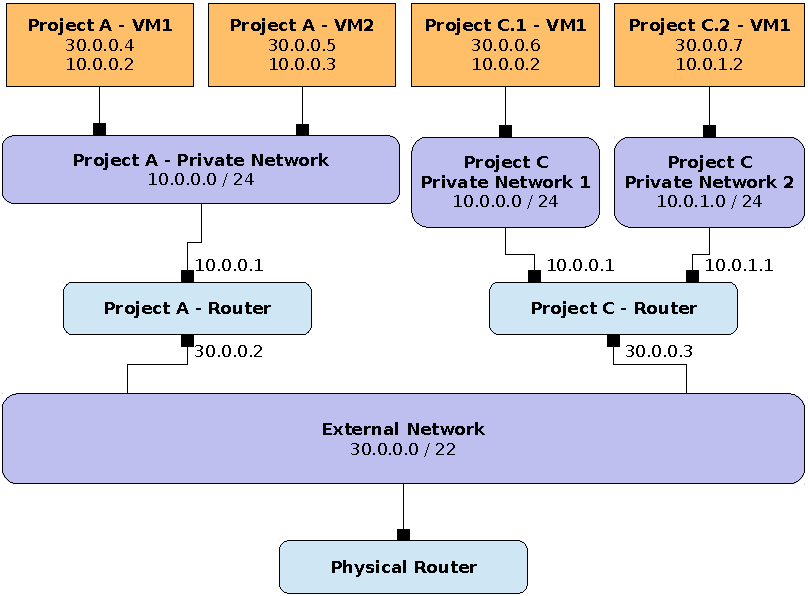
\includegraphics[width=0.9\textwidth]{imagenes/014.pdf}
 \caption{Virtual network deployment with Quantum}
\label{fig:desplieguequantum}
\end{center}
\end{figure}

\section{Compute}\label{sec:compute}

\noindent Compute is the central module. Its duty entails orchestrating the global workings in the cloud, delegating each particular function to the service on charge. In the end, Compute will let a logged user start virtual instances, which will draw their VCPU, VRAM and VHDD from the physical cluster. Yet required, Compute does not contain a virtualization package. The approach is to delegate infrastructure provision to a hypervisor found typically, but not restricted to, in the same node. To expose this on-demand computational service, Compute implements a REST API so that users can control their instances' life cycle directly from a REST client (like the CLI tools that accompany Compute).

To create an instance in effect, Compute will communicate with other modules within the cloud to orchestrate the execution and, finally, it will pass the request to the most suitable cluster node's hypervisor --- most suitable according to the cloud-defined rule set --- that will bring up the VM. Some of the supporting services are described bellow.

\begin{description}
 \item[Keystone:] Collates credentials y authorizes requests.
 \item[Glance:] Selects the OS image that will be used to start the VM.
 \item[Quantum:] Grants private and public IPs as well as manages instance network traffic.
 \item[Cinder:] Manages block storage and on-line volume attachments.
 \item[Qpid:] Handles message interchange between Keystone, Quantum, Glance and/or Cinder.
\end{description}

As it has been discussed all along, if there is some trait that aligns different IaaS Cloud implementations is their flexibility. Users' computational needs are as diverse as they are changing and therefore they expect to be given the chance to define virtual infrastructure adapting to those needs. In OpenStack, each possible particular configuration instance will take its VCPU, RAM and VHDD from a cluster host, and the users will be allowed to shape those to their requirements with ease.

\section{Glance}\label{sec:glance}
\noindent Glance is OpenStack's OS image storage service. Glance may be configured to drive images stored in a myriad of backends, ranging from Swift to an HTTP-addressable location. As happens with every other OpenStack module, Glance relies on Keystone to grant access to the images, and coordinates its operation with Compute to put them in execution on demand.

Glance supports a good number of image and container types --- this fact being merely informative to the Cloud framework as it is the hypervisor who would have to support the particular combination image type, container type ---, and they are stored as metadata linked to the image in Glance.

\section{Storage}\label{sec:almacenamiento}
\noindent OpenStack provides three main options regarding storage types:

\begin{description}
 \item[Ephemeral:] The size of the drive hosting the root file system is set following the particular flavor parameters when the VM starts. The files contained in this file system are those present in the image file stored in Glance. Any alteration to this file system will only persist the execution of the VM. Any change on the image files is written temporarily to be discarded as soon as the VM is shut down.
 \item[Block:] By making use of storage volumes managed by Cinder with \emph{LVM} (\emph{Logical Volume Manager}) OpenStack provides the ability to attach indeterminably-sized logical volumes to instances on-demand. This store kind guaranties that information is preserved between VM executions. However, this method carries an important handicap, that of being unable to attach a single volume to two different instances at the time. High availability or data safety on failure are not supported, as data is stored in a single place. A backup or RAID policies may be established to get over these limitations but they are discouraged as OpenStack has it own module to deal with them.
 \item[Safe:] Swift manages a safe distributed storage banking on controlled replication allowing for high availability deployments that overcome hard drive's inherent fragility. Swift draws on \texttt{rsync} to synchronize \emph{XFS} partitions.
\end{description}

\subsection{Cinder}\label{subsec:cinder}
\noindent Cinder es el m\'odulo de OpenStack que maneja los dispositivos virtuales de almacenamiento en bloque; de funcionalidad similar a la del \emph{EBS} (\emph{Elastic Block Storage}) de Amazon. Cinder utiliza una implementaci\'on de \emph{iSCSI} (\texttt{open-iscsi}) y LVM para Linux para gestionar las operaciones sobre los vol\'umenes. La creaci\'on, el enganche y desacople y el borrado de los bloques de almacenamiento persistente se maneja desde Horizon directamente.\newline

Estos bloques virtuales de persistencia se gestionan como vol\'umenes l\'ogicos pertenecientes a un grupo de vol\'umenes controlado por Cinder. Cinder no pretende crear un medio compartido como \emph{NFS} (\emph{Network File System}), o alguna soluci\'on \emph{SAN} (\emph{Storage Area Network}) o \emph{NAS} (\emph{Network Attached Storage}) para las instancias, ya que no es posible compartir un mismo vo\-lu\-men l\'ogico con m\'as de una m\'aquina virtual en un mismo instante. Una opci\'on interesante, que permite Cinder para facilitar ciertos despligues virtuales heterog\'eneos, es configurar las instancias para que arranquen desde un volumen creado por Cinder.


\subsection{Swift}\label{subsec:swift}
\noindent Al igual que suced\'ia con Cinder, Swift tampoco se enmarca en la idea tradicional de almacenamiento compartido en red, ni debe compararse con el anterior; Cinder y Swift cubren demandas diferentes. Se dice que Swift es ``\textit{un sistema escalable de almacenamiento de objetos, donde los usuarios registrados controlan sus compartimentos de datos o contenedores, subiendo, descargando o borrando ficheros a su antojo}'' \cite{osswift}. Funcionalmente Swift equivale al S3 de Amazon y al \texttt{Walrus} de Eucalyptus, siendo posible con\-fi\-gu\-rar un API REST compatible, parcialmente por el momento (enero 2013), con la sintaxis del primero. Una caracter\'istica fundamental para Swift es la replicaci\'on controlada.


\subsubsection{Replicaci\'on}\label{subsubsec:replicacion}
\noindent La escalabilidad, la tolerancia a fallo, la alta disponibilidad, la seguridad, el balanceo de almacenamiento y el control de carga son algunos de los rasgos que definen a Swift. La alta disponibilidad y la tolerancia a fallo se implementan usando la replicaci\'on. La replicaci\'on es un mecanismo a trav\'es del cual un sistema distribuido mantiene copias o \emph{r\'eplicas} en puntos diferentes de su despliegue, para mejorar sus prestaciones o limitar el alcalce de los fallos, entre otros.\newline

En Swift, los procesos de replicaci\'on de cada \emph{Servidor de Objetos}, que es un nodo cualquiera del cl\'uster con Swift en funcionamiento, van a comparar, peri\'odicamente, sus copias locales con cada copia remota para verificar su grado de actualizaci\'on. Cotejar estas r\'eplicas es un proceso tan costoso computacionalmente como habitual en sistemas de almacenamiento distribuido, por eso Swift se vale de estructuras como las \emph{listas Hash} o las \emph{marcas de agua} para acelerar las comparaciones. Rsync o HTTP gestionan la trans\-fe\-ren\-cia de las copias en funci\'on del tipo de objeto a replicar. La transparencia de replicaci\'on es uno de los pilares que soportan la escalabilidad de Swift. Cuando se a\~nade un nuevo nodo al espacio de almacenamiento de Swift, la redistribuci\'on de las copias es autom\'atica y, desde el momento en que \'este sea sincronizado, podr\'a responder a peticiones de datos de los usuarios.

\subsubsection{Updaters y Auditors}\label{subsubsec:otroscompswift}
\noindent Otros componentes interesantes, que completan el c\'irculo funcional descrito para Swift, son los \emph{Updaters} y los \emph{Auditors}. Los primeros act\'uan cuando se produce un error de sincronizaci\'on entre copias o cuando la carga computacional de un Servidor de Objetos es lo suficientemente alta como para que no pueda satisfacer una operaci\'on. Sucede entonces que la ejecuci\'on de esa operaci\'on se difiere; se a\~nade a una cola de actualizaci\'on que el Updater va procesando para restablecer la sincronizaci\'on. Los Auditors escanean continuamente el sistema de ficheros en busca de fallos de integridad en objetos, contenedores o cuentas de usuario, tal que, si encontrasen incoherencias, pondr\'ian en cuarentena a la entidad y pedir\'ian que se estableciese una nueva r\'eplica.
